\documentclass[11pt, pdftex, conference]{IEEEtran}
%usepackage{epsf}
%usepackage{epsfig}
\usepackage{times}
\usepackage{ifthen}
%usepackage{comment}
\usepackage{amsmath, amsthm, amssymb}
%\usepackage[margin=1in]{geometry}
%usepackage{hyperref}
\title{Lightweight Data Migration Between Clouds}
\author{\textbf{Sri Harsha Alla; Pavani Jagarlamudi, Dept. of computer science, Villanova University, 2017.}  }
\usepackage[utf8]{inputenc}
\usepackage{multicol}
\usepackage{graphicx}
%\usepackage{biblatex}

\begin{document}
\maketitle
\textbf{{\textit{Abstract --\hspace{10mm}Cloud computing services are becoming more popular as it stores large varieties of data from many applications such as YouTube, Facebook on data storage servers. However, the high concentration on lightweight data migration between clouds requires a lot of effort as each and every server has different protocols to access data. So, the devices with low computational power such as mobile devices and old generation computers cannot meet such computational overheads. In this paper, we proposed an approach by Authenticating target cloud by the user for the piece of data that is needed to migrate reduces our computation problem. From the study, an Authentication token is passed to the target cloud by using the OAuth protocol. By using the token, target cloud request the source cloud for the initiation of data migration. As a result, data that has to be migrated from source cloud to target cloud will implement minimal resource utilization of the device with low computational power. So, the mobile user’s computational overhead for the data migration between clouds will be much reduced.}}}\linebreak
\linebreak
\textbf{\textit{Keywords - Data Migration, WCF, OAuth, Token, Target Cloud}}
\section{\textbf{Introduction}}
%\textbf{Definitions}\linebreak
\begin{itemize}
\item \textbf{Cloud:} A cloud is a shared pool of computing resources which enables ubiquitous, convenient, ondemand-network with minimal effort\cite{20}. \linebreak
\item \textbf{Cloud Security:} Cloud secuirty is a set of rules and technologies to protect data, services, applications and infrastructure.\linebreak
\item \textbf{Protocol:} A protocol is defined as a set of rules and regulations that determine how data is transferred between clouds\cite{19}.\linebreak
\item \textbf{Data Migration:} Data migration is the process of sending data between source cloud and target cloud. It is a key consideration for any clpud system implementation\cite{18}.\linebreak
\item \textbf{Authentication:} Authentication is the process of establishing the truth of an attribute of a single piece of data which claimed true by an entity. Authentication involves in confirming the identity of a person by validating their identity documents or by verifying the authenticity of a website with a digital certificate\cite{17}.\linebreak 
\end{itemize}
\par
\hspace{15mm}Over the years, cloud computing has been shifting to a new paradigm. The cloud-computing paradigm provides several service models like SaaS, PaaS, IaaS to support needs of an individual or organization. The competition among cloud service providers is increasing because of increase in demand for cloud services. In such competition, clients of the cloud need to get benefited by freely and easily migrating their data from one cloud to another, which may have different environments. This data migration has to be reliable, secure, quick and at low costs.\linebreak
\hspace{15mm}The Process of Data migration is transferring data between two different clouds. There are a large variety of sensors like DHT11(a sensor to read humidity and temperature), light sensors that are used in Internet of Things and applications such as video recorders, audio recorders etc. generate large varieties of data. Where data can be an audio file, video file, document and this data can be stored in cloud storage\cite{3}. The issue is to migrate data to target cloud as quickly as possible by authenticating target cloud to obtain the best performance of the system.\linebreak
\hspace{15mm}Authentication of target cloud can be done by using Open Authentication protocol (OAuth) \cite{14}. OAuth enables an application to access each other’s data.  This protocol covers different ways to access the resources stored in resource server and works based on the roles assigned to resource owner, resource server, the authorization server and client application.\linebreak OAuth protocol works as follows,
\begin{itemize}
\item The client requests authorization from the resource owner.
\item The client receives an authorization grant that represent the resource owner's authentication.
\item The client provides authorization grant to authorization server and request for access token.
\item The authorization server authenticate the token and after successful validation provides token.
\item The client request the protected resource from a resource server by providing access token.
\item On the successful validation, the server grants an access to the resource.
\end{itemize}
\hspace{15mm}Authentication of target cloud triggers the process of data migration. Windows Communication Foundation (WCF) \cite{2} can be used for the process of data migration as WCF is compatible with communication between heterogeneous environments. WCF is a universal programming model provided in .NET framework 3.0 for building\cite{10}, configuring and deploying network and distributed applications. These applications include Message queuing and web services and many other. WCF unifies this into a single framework for both building and consuming services. WCF is a service-oriented architecture (SOA)\cite{11} and provides interoperability as the fundamental character. Because of convenient programming model but not only on its technology WCF will be the new generation development technology. As it can build future of secure, reliable and interoperable services. Though WCF have many advantages light weight data transmission is not possible because mobile device has to participate in migration.
The contributions of our study are,
\begin{itemize}
\item The major objective of the study is to reduce the burden on the mobile user over the process of data migration.
\item The protocol that is created by integrating OAuth and WCF in order to get on demand secured lightweight data migration.
\item To utilize the advantage of heavy competition in the cloud business for the cloud data storage client by migrating data.
\end{itemize}
This paper further proceeds with the following sections,
\begin{enumerate}
\item Related work
\item Methodology
\item Data Migration Risks
\item Security Issues
\item conclusion
\item Acknowlegment
\item References
\end{enumerate}

\section{\textbf{Related Work:}}
\hspace{10mm}Secure data sharing in the Cloud is a fairly new topic and has become increasingly important. The advancements, growing popularity of the Cloud and an increasing need to share data among people. Data has become the predominant factor for businesses in order to make correct decisions. So, data can have economic affect on an organization. For these reasons where clouds as data storage are emerging\cite{12}.The traditional approach for data sharing uses more computation power. Present data sharing techniques between clouds are useful to reduce the burden on the user computationally (i.e. if the user wants to migrate the data from one cloud to other then the user need not import data from source cloud and export to destination cloud as in traditional approach). These present techniques for data sharing between two clouds requires minimal interaction with the user. A few techniques that are being implemented are as follows,
\begin{itemize}
\item{\textbf{Gateway Enabled:}}
The problem with the data from the different environments can be eliminated by using a gateway in the middle for all the clouds for which data needs to be shared. As gateway provides an interface for each cloud i.e. gateway shows data of the source cloud in an understandable format of the destination cloud \cite{1}. The security problem that would be faced by using gateway is untrusted destination cloud performs insider attack i.e. similar to the known plaintext attack where destination would know the plaintext by using gateway and that can be used to attack in source cloud environment.
\end{itemize}
\begin{itemize}
\item{\textbf{Access control over connected clouds:}}
The other approach is to provide access control over the data that has to be shared between the clouds are given to the destination cloud\cite{2}. Now, the destination can initiate the data transfer depending upon the access control given by source cloud. The major problem with the approach is difficulty in organizing the data in a cloud environment as the cloud has to give access to only the data that has been requested but not all the data.
\end{itemize}
\begin{itemize}
\item{\textbf{Provide authentication for clouds:}}
In order to migrate data from one cloud to other, authentication will be given for all the end points of communication i.e. here endpoints are the source and destination clouds\cite{3}. When user requests for the data transmission, authentication tokens will be exchanged between the clouds that are involved in the data migration. Firstly, source cloud sends the metadata about the requested data to the destination cloud and destination cloud generates block access tokens. And these tokens are used to provide the authentication for the clouds which in turn provides security as only authenticated clouds are involved in the process of data migration. 
\end{itemize}
\begin{itemize}
\item{\textbf{Attribute-Based Encryption:}}
Attribute-Based Encryption is an access control mechanism, where a user or a data has attributes that are associated with it. The user should be able to access the data only if the attributes satisfy the access control policy and only if access control policy is already defined in the cloud. Attribute-Based Encryption was first proposed by Goyal et al. \cite{6}
\end{itemize}

\begin{itemize}
\item{\textbf{Proxy Re-encryption:}}
Proxy Re-encryption is a technique that is being adopted for enabling fast secure data sharing and collaboration in the Cloud. Proxy Re-encryption \cite{7} allows a semi-trusted proxy with a re-encryption key. Here, the cipher text will be encrypted with data owner’s public key and again this cipher text will be decrypted by using another user’s private key.
\end{itemize}

\begin{itemize}
\item{\textbf{ABE and Proxy Re-encryption combination:}}
ABE and Proxy Re-encryption can be combined to provide more security and privacy in the data sharing approach and provide collaboration in the cloud. Yu et al \cite{8} were the first one to combine all ABE, Proxy Re-encryption and lazy encryption mechanisms for cloud security and privacy. In this mechanism, data owner encrypts the data by using the symmetric key by using a set of attributes as KP-ABE.
\end{itemize}

\begin{itemize}
\item{\textbf{security-mediator:}}
Another approach which is simple and efficient to ensure cloud integrity without losing the individuality of the data owners and without computational overhead. So, security-mediator is introduced which will be able to generate signatures on outsourced data for data owners \cite{9}. And this have close relationship to trusted third party.
\end{itemize}
\textbf{Benefits of Data sharing:}
1. Data sharing is used for re-analyzing the problem by a researcher in a different environment that has been analyzed by another researcher in a different environment.\linebreak
2. For secondary analysis data sharing is used (i.e. data collected for one set of problems will be used to analyze the new problem which does not have data).


Xiao et al. \cite{5} identified the following concerns of Cloud computing
\begin{itemize} 
\item{confidentiality: It is defined as the assurance that sensitive information is not disclosed to unauthorized persons, processes, or devices.} 
\item{integrity: Data integrity is the assurance that digital information is uncorrupted and can only be accessed or modified by those who are authorized to do so.} 
\item{availability:It embodies the idea of anywhere and anytime access to services, tools and data}
\item{accountability:It allows the members of a cloud ecosystem to ensure that obligations to protect data are observed by all who process the data, irrespective of where that processing occurs.} 
\end{itemize}
 He keenly observed the threats to each of the concerns, as well as defense strategies.
\linebreak
\begin{figure}
\includegraphics[width=0.5\textwidth]{oauth}
\caption{Open Authentication 2.0 protocol}
\end{figure}
OAuth 2.0 is an authentication protocol which support two-legged authentication\cite{15}, where a server is assured of a user's identity. And also three-legged authentication, where a server is assured by a content provider of the user's identity. Authorization request and access tokens are assosiated with three-legged authentication. So in this paper, I would like to examine the OAuth 2.0 protocol to authenticate target cloud as an authorized user for the data that has to be migrated i.e. data owner will share his/her Auth-token to the target cloud in order to authorize target cloud and migrate data. 
\linebreak
\hspace{10mm}OAuth 2.0 protocol for authentication tokens\cite{4} works as follows,
The user accesses the client web application and clicks on login button. When the user clicks the login button, the user is redirected to the authenticating application. The authenticating application redirects the user to a redirect URI, which the client application has provided to the authenticating app. Next, the user accesses the page located at the redirect URI in the client application. In the background, the client application contacts the authenticating application and sends client id, client password and the authentication code received. The authenticating application sends back an access token.
Once the client application has obtained an access token, this access token can be sent client web application. \linebreak

\section{\textbf{Methedology}}
\hspace{10mm}We present here a secured protocol for lightweight data migration between clouds. This protocol ensures the confidentiality of user’s data while preserving their privacy. Our protocol builds on authorizing the target cloud by the user to access data from source cloud. Also, our protocol addresses the security issues that are generated by providing access to target cloud and most importantly, the computational overhead problem on the mobile users. The major protocol implementation is based on OAuth protocol for obtaining an access token to make target cloud authorized to access the data in the source cloud. When an application requests private user data, the request must be authorized by an authenticated user who has access to that data with user-centric OAuth flow. If your application doesn't need to access user data, then we should use a server-centric OAuth flow based on a service account. In our research, we need target cloud to access the user's data. So, we need to follow user-centric OAuth flow. In this methodology section, we show you the assumptions we made and detailed protocol steps.
\linebreak \par
\textbf{Assumptions:}
\begin{itemize}
\item We assume that a mobile user (user) who plans to migrate his data from source cloud to target cloud must be registered with both clouds. 
\item We assume that source cloud and target cloud applications are compatible with each other where target cloud application act as third party application between the user and the source cloud and get authorized by the user. 
\item For preserving the privacy of the user, we assume that both source cloud and target cloud do not trust each other.
\item We assume that there exists a data migration technique between clouds without user interaction.
\item And we also assume that when user requests for the redirect URL for specific data, source cloud should provide the URL that accesses only that part of data but not all.
\end{itemize}
\textbf{Protocol:}\linebreak
Initiate Data migration: The user request for the initiation of data migration in the Target Cloud (TC). In order to fetch data from Source Cloud (SC), TC application needs to get access. So, TC application requests the user for authorizing TC to access particular data in source cloud.
\linebreak
\begin{figure}
\includegraphics[width=0.5\textwidth]{CLOUD}
\caption{Secure lightweight data migration between clouds protocol}
\end{figure}
\begin{enumerate}
\item User application requests SC for authenticating TC for the particular data. In this step, the user will be waiting for the redirect URL for authenticating the user as well as TC.
\item SC application sends the redirect URL to the user. And this URL can be used only for the certain piece of data but do not permit to access all data of the user.
\item User application sends the same message which contains the redirect URL to the TC. The user need not involve in the further data migration processes because we are looking to use minimal computational power from the user.
\item By using the URL, TC application directs to authentication page and the user has to authorize the TC by providing the valid username and password for the SC.
\item SC verifies for the authorization of the user and sends the access token to the TC which have permission to access a required piece of data in SC.
\end{enumerate}
Data migration: Now TC is authorized to receive data from the SC. SC application starts transferring data to TC. And after completion of data migration, SC application invalidates the access token and terminates the whole process. \linebreak
\section{\textbf{Data Migration Risks}}
\hspace{10mm}Data migration requires data to transform its format from one system to other system. So, there are obvious risks in data migration\cite{16}.
\begin{enumerate}
\item The cut-over abort issue which may be consequence of errors in data transfer. And these about issues may even happen if data is transferred successfully.
\item Data migration issue is having the time requirements. It rarely happens that the data migration processes takes shorter than the expected time. But there is more probability that their might be unexpected delays. As the consequence, data migration may take longer time than usual.	
\item Semantic risk: Semantics of one cloud environment is different from other cloud. Semantics may be the data format or any unit as it is one of the data migration risks because of settings in two cloud applications.
\item Data corruption risk: Data corruption is case where data might be modified intentionally or due to hardware equipment that are used for transferring data which is in bits between source and target clouds. The corrupted data can make the target application to stop working accurately. 
\item Execution time: Data migration may take more time. So, in the meantime people may do serious mistakes like aborting the transmission etc. 
\item It isn't easy to predict how long data migration is going to take, nonetheless a lot of people do serious mistakes when trying to. At first, it isn't possible to scale out the time needed for transferring 1\% of data to 100\% and consider it certain. That's the most frequent cause of problems with data migration execution time.
\item Risk of losing data: Every data transfer is connected with the risk of losing a part of information. A reliable data migration requires data transferred from one source be delivered to the final destination without any losses. But, there is a possibility of losing data while data transferring from one cloud to other. In some cases this would not be a big issue but in the case of an insurance company or a banking organization etc. would lead to huge loss.
\item Data migration is not a single process and always have a set of programs and executed in predetermined order. So, one program depends on the other and that raises the risks in the data migration process.
\item Target application risks: There are the risks which are not only connected to the migration processes themselves, but also with the target application. In many cases, risks may be a matter of new application's restrictions or its incompatibility with migration programs. Even though migration seems to be really success, there is a risk that new data can harm the target system.
\end{enumerate}

\section{\textbf{Security Issues}}
\begin{figure}
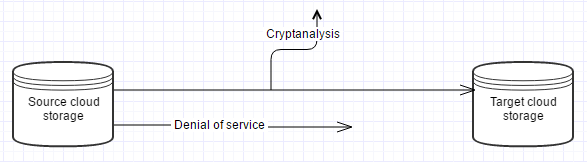
\includegraphics[width=0.5\textwidth]{cloud_issue}
\caption{Security issues}
\end{figure}
\hspace{10mm}Cloud computing is an emerging technology to which people are willing to move. So, there are obvious chances of subjecting it to some threats. 
\textbf{Threats:}
The common threats are\cite{13},
\begin{enumerate}
\item \textbf{Untrusted destination cloud:} The user wants only a specific data that need to be transferred. But while providing access tokens to the destination cloud, there is chance that destination cloud takes advantage of token to access additional data after the actual data that had transferred. This would in turn damage the security and privacy. The solution can be eliminated by providing access to a particular kind of data and token expiration. For example, when user wants to transfer the contacts from google cloud to the iCloud then google cloud upon user request provides access to the contacts of the user to the iCloud. Now, user wants to send only specific contacts then after sending those contacts google cloud should make token to expire. 

\item \textbf{Eavesdropping:} Eavesdropping is interception of a private communications, such as a phone call, and video conference by an unauthorized people in real-time. The term eavesdrop derives from some practices that standing under the eaves of a house, listening to conversations inside. Even systems that do use encryption can be vulnerable. Using a standard sniffer, user can monitor all downlink traffic. But it is difficult to monitor uplink traffic as it depends on network topology an unauthorized connection to splitters is possible and easy.
\item \textbf{Impersonation:} In order to enter a communication system, user requires to give user ID and password on the PC as an input. The hacker can use the password to make him/her as an authorized user and this is known as Impersonation. It is basically simulating a false identity. Even computers can mask against each other. So, from the beginning of the transmission to the end of the transmission it is necessary to check that each data packet really originate from the authorized user and have not been modified in middle of the transmission by an attacker. 
And there is a chance that a user in the same passive optical network will send data as another user.
\item \textbf{Denial of service:} Denial-of-service (DoS) attacks typically flood systems or networks with traffic in order to overwhelm the user’s resources and make it difficult or impossible for legitimate users to use them. While an attack that crashes a server or a system can often be dealt with successfully by simply rebooting the system. But some flooding attacks can be more difficult to recover by just rebooting the system. The United States Computer Emergency Readiness Team provides some guidelines to identify such DoS attacks:
\begin{itemize}
\item When attempting to open files stored on the network or accessing websites there can be degradation in network performance.
\item Inability to reach a particular website.
\item Difficult to access any website.
\item More spam emails than usual.
\end{itemize}
Experts recommend many strategies for business administrations to defend against a denial-of-service attack, one of them is to prepare for an incident with response plan well in advance of any attack. When a suspicious incident occur, enterprises should contact theirs ISP (internet service provider) to know whether the incident is a DoS attack or performance degradation is because of some other factor. The ISP can help to reduce the effect of attack by rerouting or throttling malicious traffic and by using load balancers.
\item \textbf{Cryptanalysis while data migration:} During data migration there is a possibility for an adversary to analyze the traffic. So, data is encrypted while data migration. There are many encryption techniques drew our attention but Attribute Based Encryption (ABE) seemed more secure. For example public key crypto-system, if the public key is receiver’s userid then sender encrypts the data based on the private key. Only receiver can decrypt the data by using his/her private key.  ABE is similar to public key encryption but a step ahead. Here in ABE, encryption is done based on the set of attributes. So, for an adversary it becomes more difficult to decrypt the message from the encrypted data. 
\end{enumerate}

\section{\textbf{Conclusion}}
\hspace{10mm} The cloud is one of the most significant shifts that computing world has gone through. The movement towards the cloud, will enable us to discover a new service based world. Where many words that were famous in the IT world like OS, servers, middleware, data centers and clustering will get erased. In order to contribute in such discoveries, we proposed a protocol which is designed by considering the following devices,
\begin{itemize}
\item Some devices cannot withstand to the high computational over heads.
\item Some devices which should not sit idle when CPU time is costlier. 
\end{itemize}
\hspace{10mm}Our protocol works to fulfill the user needs by utilizing the minimal resources from the user. The user is required only for authenticating the target cloud to receive data from source cloud. So, the user need not be idle during the data migration process. The risk of misusing the authentication can be handled effectively by the source cloud by using the technique of token expiration which eventually cause target cloud to loose authentication.

\section{\textbf{Acknowledgment}}
\hspace{10mm}We are grateful for the guidance and supervision by Prof. Henry Carter for his insightful discussions and suggestions related to the research. We also thank professor for critical reading, and for challenging the sections presented individually with commonly known solutions in the field of cloud security and privacy.

\bibliography{citations}
\bibliographystyle{abbrv} 
\end{document}
